\documentclass[../00_main.tex]{subfiles}

\begin{document}

\section{Class 15.09.2020}

\subsection{Equation of Value}

\begin{itemize}
    \item interest problems only involve 4 quantities:
        \begin{enumerate}
            \item principal value
            \item accumulated value
            \item period of investment
            \item rate of interest
        \end{enumerate}
    \item each one of them can be calculated if the other 3 are known
    \item when multiple investments are made, the time diagram is the most
        important tool
    \item then an \textit{equation of value} is set up to find the value
    \item again, be careful with interpolation between integral durations with
        compound interest
    \item finding an appropriate rate of interest such that money increases
        generally involves logarithms involves 
\end{itemize}

\subsubsection{Example 1}

\begin{itemize}
    \item Alice borrows 5,000 at 18\% convertible semiannually
    \item after 2 years, she pays back 3,000
    \item 3 years after that she pays 2,000
    \item how much does she owe 7 years after taking out the loan?
    \item time diagram:\\
        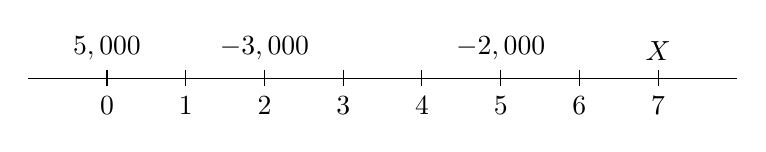
\begin{tikzpicture}
            \draw (0,0) -- (9,0);
            \foreach \x in {1,2,3,4,5,6,7,8}
              \draw (\x cm,3pt) -- (\x cm,-3pt);
            \draw (1,0) node[below=3pt, align=center] {$0$}
                node[above=3pt] {$5,000$};
            \draw (2,0) node[below=3pt, align=center] {$1$}
                node[above=3pt] {$ $};
            \draw (3,0) node[below=3pt, align=center] {$2$}
                node[above=3pt] {$-3,000$};
            \draw (4,0) node[below=3pt, align=center] {$3$}
                node[above=3pt] {$ $};
            \draw (5,0) node[below=3pt, align=center] {$4$}
                node[above=3pt] {$ $};
            \draw (6,0) node[below=3pt, align=center] {$5$}
                node[above=3pt] {$-2,000$};
            \draw (7,0) node[below=3pt, align=center] {$6$}
                node[above=3pt] {$ $};
            \draw (8,0) node[below=3pt, align=center] {$7$}
                node[above=3pt] {$X$};
        \end{tikzpicture}
    \item because the interest rate is convertible semiannually, our nominal
        rate is $i=0.09$
    \item using the diagram we see 
        \begin{equation}\nonumber
            X = 5,000(1.09)^{14} - 3,000(1.09)^{10} - 2,000(1.09)^4 = 6,783.38
        \end{equation}
    \item in the same way payments here are negative loans, withdrawals can be
        seen as negative deposits
\end{itemize}

\subsubsection{Example 2}

\begin{itemize}
    \item John borrows 3,000
    \item 2 years later he borrows another 4,000
    \item 2 years after that he borrows 5,000
    \item $i=0.18$
    \item at what time would a single loan of 12,000 be equivalent? -- at what
        time would the amount owed be the same as a loan of 12,000?
    \item draw a timeline:\\
        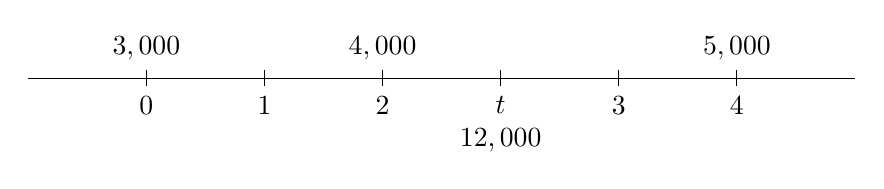
\begin{tikzpicture}
            \def\f{1.5}
            \draw (0,0) -- (\f*7,0);
            \foreach \x in {\f*1,\f*2,\f*3,\f*4,\f*5,\f*6}
              \draw (\x cm,3pt) -- (\x cm,-3pt);
            \draw (\f*1,0) node[below=3pt, align=center] {$0$}
                node[above=3pt] {$3,000$};
            \draw (\f*2,0) node[below=3pt, align=center] {$1$}
                node[above=3pt] {$ $};
            \draw (\f*3,0) node[below=3pt, align=center] {$2$}
                node[above=3pt] {$4,000$};
            \draw (\f*4,0) node[below=3pt, align=center] {$t$\\$12,000$}
                node[above=3pt] {$ $};
            \draw (\f*5,0) node[below=3pt, align=center] {$3$}
                node[above=3pt] {$ $};
            \draw (\f*6,0) node[below=3pt, align=center] {$4$}
                node[above=3pt] {$5,000$};
        \end{tikzpicture}
    \item solution:
        \begin{equation}\nonumber
            \begin{aligned}
                12,000v^t &= 3,000 + 4,000v^2 + 5,000v^4    \\
                v &= \frac{1}{1.18}                         \\
                v^t &= \frac{3 + 4v^2 + 5v^4}{12}           \\
                t &= \frac{\ln(3 + 4v^2 + 5v^4) - \ln(12)}{\ln(v)}\\
                t &= 2.11789
            \end{aligned}
        \end{equation}
\end{itemize}



\end{document}
